\chapter{On cellular signaling}
\label{introduction:introduction}

\section{Introduction}

Both in the context of multi-cellular and single-celled
organisms, cells are constantly
challenged to stay alive and perform
tasks in the face of unpredictable environmental
changes. For single-cell organisms these changes
can be particularly dramatic, as the external temperature,
osmolarity, and other properties are outside of cellular
control \cite{Bennett2008,Acar2008}.
For cells within multi-cellular organisms,
microenvironmental changes fluctuate much less due to
controlled modification of the environment by neighboring
cells. However, in order to exert control over the environment,
cells must constantly communicate with one another. The
messages sent from cell to cell are themselves a form
of unpredictable environmental change that cells must deal with.
Here, I focus on this latter problem. That is, how do
cells within multi-cellular organisms accurately interpret
messages sent from their neighbors?


The potential variety of cellular signals that cells face
is explosively large \cite{Natarajan2006},
and yet cells must somehow be able to tell these signals apart.
Mammalian cells must generally be able to respond
to changes within a highly complex biochemical milieu that contains
proteins, small molecules, and ions.
Adult stem cells must be able to reliably
divide and make differentiation decisions so as to
recreate functional units of organs. Embryonic
stem cells must be able to generate entire organisms,
going from a single cell to billions that each have different
functional and morphological properties. And those embryonic stem cells must perform this
task with extreme accuracy, since even a small error at the early
stages would be compounded through the developmental process \cite{Balazsi2011}.


It is amazing that cells can respond to such an unpredictable, complex, and
ever-changing environment. Even more amazing is that they do so
using the interactions between finite numbers
of molecules, both in quantity and type, to perform computational tasks.
In order for cells to be so responsive, they must first be
able to recognize that the environment has changed: they must have
sensors. In order for a cell to ``understand'' what has happened,
it must convert the influx of
sensory information into an internal model of its environment.
Finally, cells must map that model
onto a decision regarding what action to take in response. I refer
to the first part of this process, the conversion of external
information into an internal model, as ``signal transduction'' or, in
short, ``signaling.'' The second
part, the conversion of the internal model into a behavior, I refer
to as ``cellular decision-making.''


Understanding how cells make
decisions, as a consequence of environmental or
pathological perturbation, is at the core of cell biology.
In experimental cell biology, we purposely break the ability of a cell
to accurately process information,
or its ability to make a correct decision after processing that information,
in order to understand the
decision-making process. A cell, on the other hand, may
``unintentionally'' break those same processes, thus
resulting in pathology.
If we can understand the basis of cellular signaling and decision-making,
then we can intervene to correct such pathologies.
In this way, we hope that discoveries made in basic biology will eventually
show utility in the clinical treatment of human patients.


Cellular signaling is difficult to study, and so the degree
of uncertainty in even the best-studied systems is astonishing (as exemplified in
\ar{pathways:introduction}).
In this chapter, I outline an abstraction of the problem of cellular
signaling to give some perspective on why it is so difficult to understand.
This same abstract framework can be used to rigorously
define cell biological problems, and thus serves as a tool
for designing meaningful experiments.
By approaching the problem of cellular signal processing in this way,
we become more able to directly
answer the most basic questions in cell biology: what signals
do cells ``listen to,'' how do they model these signals internally, and how
do they use those models to make decisions?






%%%%%%%%%%%%%%%%%%%%%%%%%%%%%%%%%

\section{Canon and crosstalk}
\label{introduction:canon}

In cell biology, the big questions that we are interested in are generally imprecise.
For example, we may want to know: ``How does a
stem cell decide its fate?'' We cannot answer such questions directly, as they
are made up of an unknown number of sub-questions.
Such sub-questions that must first be addressed
include: What is a stem cell? What is a fate? And what does it
mean for a cell to ``decide''?

\subsubsection{Canon}

In practice, therefore, we typically begin with simpler and more
concrete questions, such as ``What factors influence cellular response $R$?''
where $R$ may be some property such as cell cycle arrest.
We can then screen for mutations, growth factors, or small molecules
that affect $R$, as measured using a convenient technology.
Here we are already limited in the experimental design by the variety
of the factors we have access to for testing against $R$. Further,
and perhaps more importantly, we are limited by what aspects of $R$
our technology can measure, and by not knowing whether we should even be
looking at $R$ at all.
But we must start somewhere, and so we begin to collect relationships
between experimental perturbations and measurements of $R$ for the
biological system we care about.


Over time, and across many laboratories,
we amass a library of knowledge consisting of
these experimental relationships. The meaning of each relationship alone, especially
at the beginning of the process, is fuzzy. In combination, however,
we hope that we can begin to build a model of how the biological system
works. Unfortunately, we do not know which of the perturbation-measurement
relationships are the most important, which are outright false, nor
which are only true under a particular set of experimental or biological
circumstances. We
work these disparate pieces of data into a general model
anyway, and allow that model to evolve along with our library of
knowledge, and take note of exceptions to the rules of the model. If enough
exceptions build up over time, models will sometimes emerge that can
better explain more of the data.


In the context of cellular signaling, this gradual process typically leads
to the development of so-called ``canonical'' signaling networks. These
networks are often constructed through the use of genetic experiments and
epistasis analysis, and then built upon by biochemical and other means.
Resulting canonical networks are typically depicted as protein \b{nodes} connected by
\b{edges} that carry some functional meaning, where that meaning might
be anything from the generic
``up-regulates'' to something more specific, for example an edge may mean
``phosphorylates residue $Y$, leading to ubiquitination and subsequent
degradation.''


Historical happenstance and available methodologies therefore play a large role in
how we define
canonical pathways. In cell and molecular biology education, we are often
taught cellular signaling through these canonical pathways
via the key experiments that laid their
foundations. We are therefore trained from the beginning to see the pathways as
non-overlapping, distinct channels of information
within cells that each carry out prototypical functions.


\subsubsection{Crosstalk}

However, once a canonical framework is in place, and is
generally accepted throughout the field, new findings must still
be attached to that framework. In this way, canonical networks tend to
continuously expand, eventually encroaching onto territory that once
belonged to some other canonical pathway
(see \ar{fig:introduction:complexity})  \cite{Kholodenko2006}.


  \begin{figure}[!bt]
  \centering
  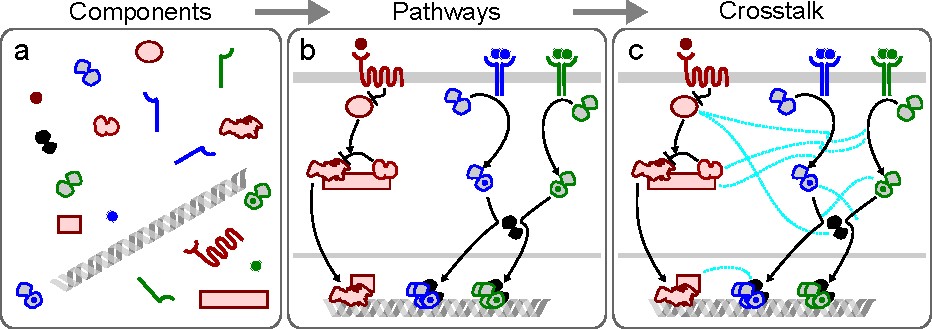
\includegraphics[width=6in]{FIGS/introduction/complexity.pdf}
  {\singlespacing 
  \caption[ Apparent signaling complexity increases over time.]
            { Apparent signaling complexity increases over time.
			\b{a}, Components of signaling pathways are typically discovered by
			genetic means or by treating cells with unknown, purified factors and
            observing the resulting phenotypes.
			\b{b}, These components are then organized into canonical signaling
			pathways based on epistasis experiments. \b{c}, Finally, canonical pathways
			are interconnected by new experiments whose results
			do not fit into the canonical framework. The network edges, as drawn here,
            may each have a different meaning and may be specific in time or to
            certain experimental contexts.}
  \label{fig:introduction:complexity}}
  \end{figure}


As canonical pathways send more and more tendrils into the global network,
we end up with models of cellular signaling wherein any perturbation
to the system ends up reverberating throughout the entire web: everything is
connected to everything. I refer to this phenomenon generally as ``crosstalk.''
While one may wonder how we can begin to address
such complexity, it is possible that the situation is less complex than we think.


An important aspect of these networks that is all too frequently ignored 
is \textbf{time}. The models that are sketched out
in any good review are static approximations of the true signaling
network. In effect, these static
networks are the maximum projections of a set of networks that exist across time
and across different experimental conditions. The actual network, evolving dynamically within
a cell as it processes information, might not ever look like the static map \arp{fig:introduction:xtalk}.


It is a rare experiment indeed that
measures all of the network edges simultaneously, as the goal
of most experiments is to flesh out a single edge or node. Therefore
we do not generally know if a given edge or node exists at all times, in all
systems, or if it is instead an ephemeral thing that comes and goes
as needed. Indeed, experimental evidence has demonstrated that the topologies of
signaling networks may not be constant, and that they may be
relatively simple at any instance in time \cite{Ideker2012,Ku2012}.


Aside from the missing temporal aspect in our static canonical networks
and inter-networks, there is another important and oft-ignored aspect.
That is, an edge is only useful for signaling if it
somehow transfers \b{information}. The purpose of a biochemical
signaling pathway is to carry information from one node to another.
The fact that two nodes are connected by a link, one that perhaps indicates binding
or phosphorylation, does not imply that information has been transferred.
Some edges between nodes may be tangential to the signaling process being studied,
or may be sending information into parallel signaling channels.
This information content problem should become clear later in this chapter and
in the particular case of signaling crosstalk reviewed in \autoref{pathways:introduction}
and studied in \ar{insulation:introduction}.


Instead of continually adding inter-network
edges, perhaps then we should carefully evaluate the edges
that already exist. By testing those edges across systems, at different times,
and explicitly verifying that they carry information, we may find that
some of these edges carry little weight and that therefore our
currently-complex view of signaling
must be both simplified and made dynamic in order to reflect reality.


  \begin{figure}[!bt]
  \centering
  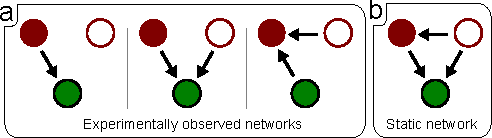
\includegraphics[width=4in]{FIGS/introduction/xtalk.pdf}
  {\singlespacing 
  \caption[Static networks may not represent true network behaviors.]
            { Static networks may not represent true network behaviors.
            \b{a}, Networks collected from multiple experimental conditions
            may show a variety of topologies. \b{b}, The static network
            diagrams that we typically draw are maximum projects or averages
            across the various experimentally observed topologies.}
  \label{fig:introduction:xtalk}}
  \end{figure}

\section{Cells as functions}
\label{introduction:hierarchy}

Abstracting cell biological systems into mathematical or computational
models can be a powerful way to learn about those systems, though the
value of any given model can vary tremendously. If a model is as
complicated as the system it represents,
we have learned nothing; if the model is too simple, we have not captured
the biology we are trying to understand. In any case, the process of modeling
itself brings a rigor to and an awareness of the studied system that might not have
otherwise been possible \cite{Janes2013,Zhang2013,Pe'er2011}.


This section is primarily intended for classically trained
biologists, like myself, who are not often exposed to this way of thinking.
Those in fields that are historically more modeling-oriented,
such as computer science and systems biology, will likely find the following
to be familiar.


\subsubsection{Setting up an abstraction}


A useful abstraction when developing models of
cell signaling is to think of cells
as functions $f$ that convert sensory inputs $S$
into behavioral responses $R$, such that $f(S)=R$. For example,
$S$ may be the concentration of an extracellular ligand, while
$R$ may be the nuclear concentration of a downstream
transcription factor, so that $f(S)$ models the
behavior of a receptor that converts one to the other.
The function, then, is typically the biological process that we wish
to understand.


I borrow the term ``encoding'' from computer science
to refer to this relationship, because it carries with it the
idea that it is \b{information} that is being converted from one form to another.
Using this language,
$f$ encodes $S$ into $R$. Take human speech as an example. 
In speech our brains generate
words that are encoded into complex temporal patterns of
vocal chord tension, lung contraction, tongue movement, and so
on. Those patterns in turn encode temporal changes in air
pressure that propagate away from the speaker. Cells
in the ear of the listener encode those pressure changes into
mechanical movements, which then encode those movements into
neuronal activity that the listener finally decodes into the
original spoken words.


For experiments in this framework, $S$ is whatever
experimental perturbation is being applied, $R$ is the
experimental readout, and $f$ is the biological encoding process that
we are trying to understand. The assumption in our experiments,
then, is that knowledge of $S$ and $R$ are sufficient to infer
$f$. When we first dive into the complete unknowns of a
phenomenon, a precise inference is essentially impossible.
As a consequence, we find ourselves using vague
words to describe $f$, such as ``recruits,'' ``activates,''
or ``mediates''; the function remains a mystery.


For values of $S$ and $R$ that are
closely connected by some process, experiments allow us
to associate more precise
mechanisms with $f$, so that we can describe the function with words like ``binds''
or ``phosphorylates.'' However, for values of $S$ and $R$
that are distantly connected, perhaps through other nodes such as in the 
case of speech described above,
clear definitions of $f$ become more difficult. This
is a constant struggle in the study of developmental signaling pathways,
as studied in this dissertation, because many of their
interesting biological effects are far removed in time from the
signaling event. Activation of these pathways may therefore
induce many complex layers of signal processing before finally affecting $R$
\arp{fig:introduction:function}: the function is a composition of functions.


To precisely model mechanism in such cases, collapsing the
relationship between $S$ and $R$ into an understandable function is impossible.
Instead we would need to break the original function into many, where
the output of each function becomes the input for the next
(\ar{fig:introduction:function}), and study them individually.
By breaking up a general, indirect model (e.g. ``Wnt blocks
stem cell differentiation'') into a set of more specific models with direct
relationships (e.g. ``Wnt binds Frizzled, resulting in
increased \bcat, which in turn binds to the Myc promoter and
increases its expression''), we obtain insight about mechanistic details
at the cost of simplicity.


  \begin{figure}[!bt]
  \centering
  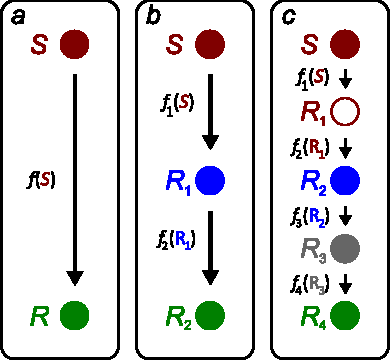
\includegraphics[width=2.5in]{FIGS/introduction/function.pdf}
  {\singlespacing 
  \caption[Abstracting signaling as a hierarchy of functions.]
          { Cells can be abstracted as functions that take sensory
			inputs $S$ and yield output responses $R$. However, interpretation of this
			abstraction suffers from unknowns between the initial
			input $S$ and the final output of interest $R$ (\b{a}). By adding
			more (\b{b}) and more (\b{c}) components the model becomes
			complex but each link gains functional insight.}
  \label{fig:introduction:function}}
  \end{figure}


  
As an additional point, for a given biological function $f$ there can be
multiple inputs and outputs, many (or most) of which are unknown.
And so the inputs and outputs are better thought of
as lists or vectors, as in equations
\ref{eq:introduction:inputs}-\ref{eq:introduction:function}
(bold face, non-italics indicate a vector).
In this model, the true
values of $\vec{S}$ are the known and experimental parameters
as well as any unmeasured parameters
(e.g. $S_1$ to $S_3$ may represent treatment duration,
treatment concentration, and ambient temperature). The values
of $\vec{R}$ are the measured responses as well as any unmeasured
cellular parameters that change in response to $\vec{S}$.
To complicate
matters, each parameter may have completely different units
(e.g. concentration versus temperature).
We must inevitably approximate the true
biological parameter vectors $\vec{S}$ and $\vec{R}$
by choosing a small known subset of their values, and
thus can only ever obtain estimates of the true function $f$.
%
    \begin{gather} 
    \vec{S}  = [S_1\cdots S_n] \label{eq:introduction:inputs} \\
    \vec{R}  = [R_1\cdots R_m] \label{eq:introduction:outputs} \\
    f(\vec{S})  =\vec{R} \label{eq:introduction:function}
    \end{gather}


Aside from the obvious issue that our approximate
models can only include things that we know about, cellular functions are often highly
non-linear. That is, it need not be true that $f(S_{1a}+S_{1b})=f(S_{1a})+f(S_{1b})$,
where $S_{1a}$ and $S_{1b}$ are different values for the same parameter,
nor that $f(aS)=af(S)$, where $a$ is a constant. A typical dose-response
curve makes a good example, since doubling the dose
(by setting $a=2$) does not necessarily double the output (i.e. $f(2S)\neq 2f(S)$).
Temporal feedback makes the models even more complex, since this 
allows a function to eventually modify its own input.
	

\subsubsection{Making use of the abstraction}


To summarize, we can think of cells as
hierarchies of functions, where the true signals $\vec{S}$ and responses $\vec{R}$
make up the nodes
of a signaling network, and the functions are the mechanistic activities that
connect them in time. The functions we study may take into account
many parameters of which we are completely unaware, and so we only obtain
estimates of $f$. Our goal in studying cell signaling is to estimate $f$
as accurately as possible, so that $f(S)\approx f(\vec{S})$.
Finally, to be able to assign a clear functional meaning to
a particular $f(S)=R$ relationship,
$S$ and $R$ must be closely connected.


A common approach to modeling signaling pathways,
that allows for both non-linearity and temporal feedback, is to assemble systems
of ordinary differential equations for
every known node and edge in the network and to explore the behavior
of the system computationally. Even a small non-linear network
can generate a wide variety of outcomes given different parameters
or small changes in topology
\cite{Shoval2010a,Wang2013b,Goentoro2009,Kholodenko2006}. Therefore, we can test
the completeness of our understanding of a signaling pathway by, for example,
testing the robustness of the model's output
against a wide array of biologically reasonable parameters (analogous to experimental
perturbations). Such approaches can
uncover deficiencies in our knowledge, as the fragility or
failures of the model may indicate a missing function or node.
Unfortunately, it is not true that successful recapitulation of a biological behavior by a
mathematical or computational model implies that we have captured
the true biology with that model.


Given the potential complexity of biological signaling models, and
the high likelihood that any given model is incomplete or flat-out
wrong, what is the value in developing models at all? I have already noted
that models give us the
potential to identify deficiencies in our knowledge, and
that building models forces us to rigorously define the questions
we seek to address. There is an additional important benefit, which is
that models may allow us to uncover underlying simplicity.


If a model
is built that recapitulates a biological phenomenon, then parts of
the model can be removed in order to determine the minimal set of
components that could create the observed biological behaviors. Having identified
these nodes one can convert a complex mechanistic model into a simple conceptual one
\cite{Ku2012,Dutkowski2011}. Additionally, if a behavior can be represented by
a highly simplified version of the functions that cause it, we can begin to
ask why the system is more complicated than it needs to be. We must be
careful with such ``why'' questions, since biological functions are created
via a random evolutionary process. However, such questions can
lead to biological insights about benefits to regulation or signal processing
of the more complex observed signaling network.

  



\section{The information encoding problem}
\label{introduction:encoding}


An analogous problem to the one we face when trying to understand
cell signaling is the following.
Going back to the example of human speech, how would
alien scientists with no concept of sound think that we
communicate? Perhaps they would observe us over long periods of time, 
and eventually correlate certain patterns
of mouth movements by one human to some behavioral task
performed by another. These aliens
might quite reasonably infer that we encode
communicated messages into mouth movements that are then decoded visually
by the recipient.


Indeed, that putative encoding is a reasonable
approximation of the true encoding, largely because mouth movements
are part of the encoding process that is used by the full sound-based
encoding. This is, of course, why humans can learn to accurately ``read lips.''
Some of these alien scientists would eventually notice that we can
still communicate in the dark, and claim that this discovery shows that
the original encoding model was incorrect. Importantly, breakdown of the model
in this context did not mean that it was incorrect, it simply meant that
some part of the message was being carried through an additional, unobserved channel (sound).


We face the same issue when trying to identify $\vec{S}$ and
$\vec{R}$ for studying cell signaling. Communication via molecules
is so outside of our experience that we have no choice but to make
educated guesses as to how it might work in each context.
There are many approaches for converting biological
data into models, but how do we know what the relevant data
are? In the broad sense, the relevant data are whatever the
cell ``cares about.'' Unfortunately we neither know what
signals a cell is listening to, nor into what form it encodes
this information. If we don't know $\vec{S}$, and
we don't know $\vec{R}$, how can we possibly determine $f$?
I refer to this generally as the ``encoding problem.''


\subsection{Identifying inputs and outputs}


The first difficulty we face is the determination of $\vec{S}$. 
We frequently assume that the property
of signal that the cell cares about is its
concentration (as for a ligand or drug) \cite{Becker2010,Cheong2011}.
From a biochemical perspective this is a sensible guess for what
is being encoded, since we understand biology as a collection of
intermolecular interactions that have binding constants, may show
cooperativity, and that have behaviors that fit onto Hill curves.
This leads to the further expectation that the
input concentration is saturable, following some form of a sigmoid
curve. The assumption that cells sense absolute concentrations need not
necessarily hold true, however, as various pathways can instead show fold-change
detection \cite{Goentoro2009,Shoval2010,Lee2014}. Further, responses need
not follow typical sigmoid curves, as they can sometimes show linear responses 
over a large range of concentrations \cite{Becker2010}.


For $\vec{R}$, we often make a similar assumption that cells encode the
received signal into intracellular concentrations of some factor.
Indeed, this concentration-based encoding defines
morphogenic signaling, which
is typically thought to convert external ligand concentrations into active transcription
factor concentrations. But again the concentration property need not be
the value of $R$ that encodes the sensory input.


For example, the Tumor Necrosis Factor/Nuclear Factor
kappa B (TNF/NF-$\kappa$B) pathway
does show ligand concentration-dependent increases in its nuclear transcription
factor accumulation, but in such a noisy way that single cells may not be able
to accurately sense the absolute ligand concentration \cite{Cheong2011}.
This implies either that single cells are
poor signal processors or that, alternatively, the absolute ligand concentration only
partially encodes the information that the cells are using.
The latter may be the case,
as recent work indicates that the information content of TNF
concentrations is more accurately encoded into the fold-change of transcription
factor activity \cite{Lee2014}.


Another alternative to encoding to or from molecule concentration is the use of
temporal information, such as integration over time or oscillatory behavior
\cite{Tay2010,Kang2011}. Therefore, care should be taken with the assumption
that absolute concentration is of utmost informational value to the cell. This assumption
is difficult to test, however, as there may be a concentration dependence
even if this is not the primary encoding that the cell uses,
as is the case for TNF/NF-$\kappa$B signaling and for the analogy
of mouth movements in human speech.


\subsection{Cellular variability}
\label{introduction:variability}

For a given approximation of $\vec{S}$ and $\vec{R}$,
is it fair to assume that this approximation is equally meaningful
for all cells in the population? Most of our knowledge of signaling stems
from population-based measurements of cellular responses, for example from
Western blots, microarrays, and other common cellular lysate-based
methods. Such methods yield averaged cellular behaviors, therefore
making the implicit assumption that this average reflects individual
cell behavior \cite{Snijder2011,Altschuler2010,Huang2009}.
If this assumption is incorrect, such that our measured values of $R$
do not reflect any real cellular behaviors,
then the properties of $f$ that we infer will be incorrect.


Indeed, many studies have shown that this assumption of cellular homogeneity
is unjustified. Dramatic examples include the classic demonstration
that single \frog\ embryos have switch-like instead of graded
behavior \cite{Ferrell1998}, the finding that various factors thought to be correlated
during adipocyte differentiation were only correlated in a small
subset of cells while being anti-correlated in others \cite{Loo2009}, and the
discovery that
population-averaged measurements were hiding the ultra-sensitivity
of temporally asynchronous bacterial motors \cite{Cluzel2000}.


How can single cells display behaviors different from the population average?
Take the trivial case: a tissue sample may include many different cell types
that have quite different properties. For example, the intestinal
epithelium contains highly-secretory goblet cells and highly-absorptive
enterocytes, but the average behavior of these cells might be neither secretory nor
absorptive. In a less
trivial case, single cells within an apparently homogeneous
cultured cell line can also exhibit cell-to-cell differences,
even if they are derived from the same clone \cite{Singh2010}.
Such within-cell type differences could be due to asynchrony in cell cycle position
\cite{Sigal2006a} or to asynchrony of other phenotypic states
\cite{Kobayashi2009,Kalmar2009,Tay2010,Loo2009}.


Cultured ``homogeneous'' populations can thus show single-cell variation due to an
asynchrony in temporal movement between stable phenotypic types, but they
can also vary more stochastically. Randomness in cellular phenotypes
might stem from asymmetry in inherited properties after stem cell
division, for example \cite{Spencer2009,Navarro2012,Chang2008,Kalmar2009}. 
Additionally, because genes are
typically present in only two copies, and a finite number of molecules
mediate the process of transcription, it is necessarily a noisy
process \cite{Elowitz2002,Munsky2012,Sanchez2013} that can also generate
cellular variability. Note that, without careful temporal studies, variation
due to asynchrony in stable states cannot be easily differentiated from
that due to rapid movement between unstable states.


Outside of fully distinct cell types, why do cells display such variability?
There is no clear answer to this question, though there are many potential
explanations. Perhaps the use of molecules to process information is simply
so inaccurate that it must generate extensive noise. Maybe cells can work
around the noise we that see, so that their behaviors are more precise
than they appear. Or perhaps cells have
adapted to deal with such noise by either suppressing
or making use of it. Indeed, in some cases variability
can be useful to the population \cite{Eldar2010}, as single cells may generate
subpopulations with useful functions. An example is cellular
differentiation in mammals, where stem cells need to choose whether to
differentiate, and to which fate \cite{Chang2008,Kalmar2009,Navarro2012}. In other cases
subpopulations may have resistance to toxic
environmental stresses \cite{Veening2008,Slack2008,Singh2010}, though we
should be cautious with just-so explanations for these kinds of links.


\subsection{Context-dependency}
\label{introduction:encoding:context}

Transcriptional
networks and chromatin state are highly cell type- and
environment-dependent. As a consequence, properties that are essential
to signaling may vary between experimental systems. Examples include
concentrations of cellular receptors, pathway
modulators, and effectors. Such
differences in cellular properties and in the microenvironments
in which cells live are often collapsed into the term ``cellular context.''


Cellular context also includes properties
of other signaling pathways, which is important because
canonical pathways may be not be isolated information channels.
Thus, knowing the likely extent of crosstalk
is important, though general pathway interconnectedness is
difficult to measure. Some types of signaling are particularly interconnected,
such as for the growth factors that modulate
downstream kinase cascades due to the use of higly overlapping downstream components
\cite{Janes2006}. On the other hand, other pathways
may be much less interconnected, as I show in this dissertation
for several key morphogenic signals \arp{insulation:introduction}.


Attempts to quantify pathway interconnectedness are few and are
necessarily limited by what can be practically measured, along with the issues I
have already noted in this section.
Computational work seems to show that signaling through one
pathway can be broadly modulated by properties of the entire
cell signaling network \cite{Domedel-Puig2011}, while experimental
work shows that non-additive inter-pathway crosstalk is a sparse phenomenon
even for high-order combinations
of up to five signaling pathways \cite{Natarajan2006,Hsueh2009}.



\section{Solving the encoding problem}
\label{introduction:encodingSolution}

I have painted an admittedly bleak picture of the difficulties in studying
cell signaling. It should be clear from this discussion that experimental
design in cell signaling is quite difficult, and interpretation of experiments
must be done with extreme care. But can we remove, or at least reduce,
some of the difficulties discussed above?


\subsubsection{Obtaining meaningful $S$ and $R$}

Perhaps the most problematic of the issues discussed is that
of not knowing which signals $\vec{S}$ a cell is interested in 
nor which responses $\vec{R}$ encode those signals. One can begin to address
this by considering different variations of the inputs (e.g. changing
concentrations or treatment durations) and outputs
(e.g. phosphorylation states, live-cell measurements of the same
cell over time, fold-change in concentration, total change in concentration).
Further discussion of different output measurements, in the particular
context of single-cell fluorescence microscopy, can
be found in \ar{imaging:introduction}.


Assuming that one could identify a series of potential input signals
and response metrics, it is not obvious how to go about identifying
which are the more accurate estimates of $\vec{S}$ and $\vec{R}$.
An interesting
approach would be to perform measurements of information content
between putative combinations of $S$ and $R$, for example using the
mutual information metric \cite{Cheong2011}.
Under the assumption
that the cell is encoding signals in the most informative way
possible, the $R$ and $S$ choices that maximizes mutual information can then
be considered to be the best approximation
of the encoding that the cell uses. This would require either high
accuracy in measurement or precise knowledge of measurement error. 
In \ar{insulation:introduction} I test multiple reagents and readouts
to ensure that they have similar information content, and I discuss
this approach in more detail in
\ar{imaging:introduction}.


In an example of this approach, research groups measured the
information content of transcription factor gradients across
\fly\ embryos, with the question of whether enough information
was present to specify the location of all nuclei along the embryo.
While each transcription factor had low positional information content when taken alone,
in combination the factors did have enough information to specify each nucleus
position with high accuracy \cite{Gregor2007,Dubuis2011,Dubuis2013}.


As with the example of human speech above, 
it is important to remember that low information content of a
single $S$ does not
necessarily mean that it is an \i{incorrect}
encoding. It may alternatively signify an \i{incomplete} encoding,
and that that other unmeasured signal properties need to also be considered.
Importantly, incomplete encodings can be good enough for many
experimental biology questions.



\subsubsection{Compensating for cellular variability}


To address issues stemming from cellular variability, the
straightforward solution is to directly measure its effects on the
experimental relationship between the chosen $S$ and $R$. Measurements
of $R$ can be performed on a single-cell basis, for example by
microscopy (as in this dissertation) or by flow sorting.
The distributions of single-cell values can then be checked for properties,
such as multi-modality, that would suggest the presence of multiple
cellular states. (In my work (\ar{insulation:introduction}),
I verified that each measurement generated unimodal single-cell distributions.)


In the case that different cellular states do exists, each cell
can be grouped into statistically distinct subpopulations by measured
phenotype \cite{Loo2010,Singh2010}. Each subpopulation can then be
tested separately to see if each has the same $f(S)=R$ relationship.
For example, in \ar{insulation:introduction} I test how cell cycle phase
affects measurements of inter-pathway crosstalk. Further, if live-cell markers
are able differentiate subpopulations, then cells can be physically
sorted and experimented on separately.


Importantly, the absence of subpopulations
along the dimension of the measured response $R$ does not imply that
all cells are the same. Rather, it implies that we cannot claim that they
are different. Conversely, the presence of subpopulations in one
dimension does not imply existence of the same subpopulations with respect
to other dimensions (see \ar{fig:introduction:subpops}). In other
words, the presence or absence of cellular subpopulations as measured
by one readout is insufficient evidence to make a claim about whether $R$
is being distorted by the presence of subpopulations. Such a connection
must be explicitly tested.


  \begin{figure}[!bt]
  \centering
  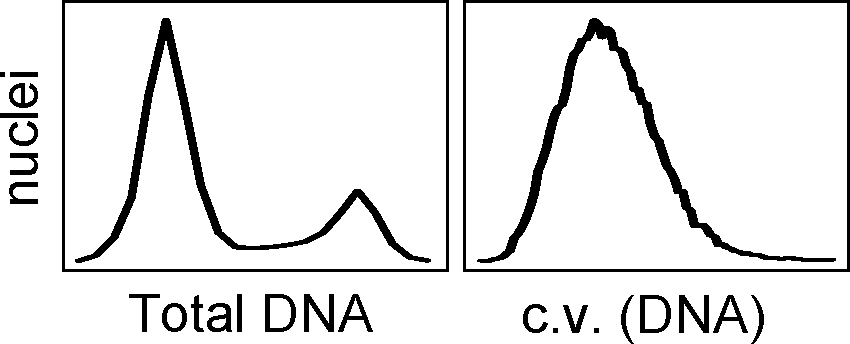
\includegraphics[width=2.5in]{FIGS/introduction/subpops.pdf}
  {\singlespacing 
  \caption[Cellular subpopulations are phenotype-dependent]
          { The presence of subpopulations in one measurement dimension
            does not imply subpopulations in another dimension;
            subpopulations are a phenotype-dependent property.
            (\b{a}) Cells show bi-modality in their total DNA content
            (as measured by total Hoechst fluorescence), but 
            (\b{b}) not in the coefficient of variation in DNA content.
            These measurements are addressed fully in \ar{imaging:introduction}.}
  \label{fig:introduction:subpops}}
  \end{figure}



\subsubsection{Determining context-dependency}

Finally, how can we deal with the issue of context-dependency?
First, it is important to verify that the context-dependency truly exists.
As I discuss in \ar{pathways:introduction} and implied in this chapter,
context-dependency of biological phenomena is often inferred by
the fact that different labs produce different results when asking
the same questions. However, interpretation of cell signaling results
are incredibly complicated, which may
simply mean that the labs were not, in fact, asking the same questions.
Because cells
may be encoding information differently than we expect, we should
take care when comparing interpretations of results obtained by different
experimental methods, as each method will approximate $\vec{S}$ and $\vec{R}$
differently.


However, some (perhaps much) of context-dependency is undoubtedly
real, and can be absorbed into the simple model of cells as functions.
While we could allow the function to vary from context to context,
it is more useful to say that $f$ does not change but that
subsets of the inputs $\vec{S}$ and outputs $\vec{R}$ can vary.


To get around this parameter variation, we can first make sure that
all controllable conditions are kept the same and that all measurements
are the same from experiment to experiment. Thus, the experimentally-defined
subset of values in $\vec{S}$ and $\vec{R}$ do not change. Experiments can
then be repeated identically across multiple cell types, so that the only
varying parameters are those inherent to cell type differences.
Any consistent aspects of the relationship between experimental
$S$ and $R$ across diverse cell types can then be used to infer the
general properties of $f$. Indeed, this approach is common in cell biology,
as it is widely believed that any given cell line may have a myriad of
idiosyncratic properties.


When using such a multiple cell-type approach, one may find a case
where context-dependency is so dramatic that no
general properties of $f$ can be uncovered. The first aspect
of this problem to tackle would be to carefully ask if the cell types
are truly being treated ``identically.'' As suggested above,
experiments typically use an absolute set of conditions across cell types
(e.g. identical ligand or drug concentrations). But it may be the case that two cell
types simply vary in sensitivity to the conditions, such that one type
is effectively receiving a half-maximal dose while the other is saturated.
Because we do not know which property $R$ encodes the treatment condition,
it is also difficult to know if we are measuring an ``identical'' readout.
Perhaps some of the apparent context-dependency of signaling is due to
incorrectly interpreting what it means to treat different cell types
identically.


Instead of relying on constant treatment concentrations
derived from the literature and applying such conditions generally
across experiments, another approach would be to measure dose-response and time-response
curves for all cell types that are under experimentation. Conditions could then be
calibrated on a cell type-specific basis so that, for example, all cell
lines receive a half-maximal input concentration.


\subsubsection{The encoding problem is unsolved}

Part of the intention of this chapter was to make it clear that
cellular signaling is an incredibly difficult phenomenon to understand,
and that experimental designs are making many
assumptions that are either going unnoticed or are not
being made explicit. Some of these assumptions, if made explicit, might
dramatically affect how we interpret our experimental results.


There is no general solution to the encoding problem but,
as I have outlined here, steps can be taken to minimize its effects. Perhaps more
importantly, an awareness of the assumptions allows for them to be tested
in some cases or, at minimum, allows for results to be interpreted cautiously
in the light of those assumptions.



\section{Dissertation aims}
\label{introduction:aims}

This chapter provided an abstract foundation on the
problems faced in the study of cellular signaling. In particular,
I focused on our lack of clear knowledge about how cells encode signals into
intracellular models, and how this lack of clarity may
be leading us to unnecessarily complex signaling pathways.
In this dissertation I present a case study of one
such apparently-complex signaling phenomenon, that of
cross-pathway integration between Wnt and Transforming
Growth Factor Beta signaling, wherein I demonstrate that the
interactions are simpler than is currently believed.


In \ar{pathways:introduction} I review the literature on the 
classic developmental signaling
pathways that are the focus of my case study, and the
claimed mechanisms off crosstalk between them.
These are the Wnt and
Transforming Growth Factor Beta pathways. I chose these signaling
networks because they are highly studied, and so have
well-established approximations of what cells care about both for inputs
$\vec{S}$ and outputs $\vec{R}$. Further, both Wnt and TGFB have
relatively clean canonical forms that do not share any core
components, and yet there is a large body of work that
ties these pathways together.


In \ar{imaging:introduction} I establish rigorous, quantitative methods for fluorescence
microscopy image analysis that I use to study crosstalk
between the Wnt and TGFB pathways. The study of crosstalk requires
a large number of experimental conditions, and the literature on 
crosstalk generally lacks single-cell resolution. I therefore chose high-throughput
immunofluorescence microscopy as my primary experimental method.
Precise single-cell measurements
are essential to quantifying single-cell
phenotypes, and so I focus on the discussion on how experimental
error can be removed or measured.


In \ar{insulation:introduction} I make use of the conceptual approach to
cellular signaling described in \ar{introduction:introduction},
the body of literature about the Wnt and TGFB signaling pathways
reviewed in \ar{pathways:introduction}, and the quantitative methodologies
established in \ar{imaging:introduction}, to experimentally determine
the degree of Wnt/TGFB crosstalk during signal transduction. There, I
demonstrate the finding that these pathways are in fact insulated from
one another, thus making a case for simplicity in morphogenic signal
integration.


\subsubsection{Reading this dissertation}


Each chapter is relatively independent, though
the reader may find some points confusing without reading earlier
chapters. \ar{imaging:introduction}, on quantitative single-cell imaging,
in particular can
stand alone and so I have placed it near the end so as to not disrupt
the flow of the biological content of Chapters \ref{pathways:introduction}
and \ref{insulation:introduction}.
The imaging chapter should be a useful guide to any biologist or analyst
in need of a conceptual and practical reference for rigorous image analysis.
Those readers primarily interested in the biology of Wnt and TGFB signaling
crosstalk can skip \ar{imaging:introduction} without significant loss of coherence.

